% Capítulo 2, Fundamentação Teórica
Este capítulo consolida a base teórica e técnica da pesquisa, descrevendo as restrições fundamentais dos sistemas distribuídos e seus modelos de consistência com a arquitetura prática dos \emph{In-Memory Data Grids} materializada pela plataforma Infinispan. A validação estrutural desse ambiente concorrente é explorada por meio das técnicas de especificação formal e \emph{model checking} com TLA+, cuja garantia a priori é complementada pela análise do comportamento dinâmico do sistema através do estudo da latência de cauda e da definição de Objetivos de Nível de Serviço (SLO). A estabilização dessas métricas operacionais recorre aos princípios teóricos de sistemas autoadaptativos e controle por realimentação, estratégias de mitigação que culminam na caracterização do domínio prático da gerência de sessão sob normativas de segurança.

\section{Sistemas distribuídos: consistência, replicação e falhas}
\label{sec-fund-distrib}

Um sistema distribuído é um conjunto de processos sequenciais que se comunicam por troca de mensagens, sem relógio global comum. Para raciocinar sobre as execuções desse sistema, \citet{lamport_time_clocks_1978} introduz a relação de precedência causal, denotada $\to$, definida como a menor ordem parcial irreflexiva que satisfaz duas regras: se duas ações $a$ e $b$ pertencem ao mesmo processo e $a$ ocorre antes de $b$, então $a \to b$; e se $a$ é o envio de uma mensagem $m$ e $b$ é o seu recebimento, então $a \to b$. A relação é transitiva, e dois eventos $a$ e $b$ não ligados por $a \to b$ ou $b \to a$ são considerados concorrentes, denotados $a \parallel b$. Para tornar essa ordem parcial observável em cada processo, o algoritmo de relógios lógicos atribui a cada evento $a$ um valor inteiro $C(a) \in \mathbb{N}$ que respeita a precedência causal, ou seja, $a \to b$ implica $C(a) < C(b)$. Cada processo incrementa seu relógio a cada evento local e, ao receber uma mensagem $m$ com marca de tempo $C(m)$, atualiza o relógio para $\max(C(p), C(m)) + 1$, o que mantém a contagem coerente com as mensagens recebidas. Essa construção é a base sobre a qual modelos de consistência são definidos como restrições sobre quais ordens totais dos eventos são admissíveis como observação externa do sistema.

A literatura distingue uma hierarquia de modelos com garantias decrescentes. A linearizabilidade, definida por \citet{herlihy_wing_linearizability_1990}, exige que toda execução concorrente seja equivalente a alguma ordenação sequencial das operações que preserva a ordem temporal de operações não sobrepostas: se a resposta de uma operação $a$ ocorre antes do início de $b$ em tempo real, então $a$ precede $b$ na ordem sequencial equivalente. Cada operação tem efeito em um único instante situado entre sua invocação e sua resposta, e o efeito visível corresponde ao de uma cópia única do objeto. Duas propriedades adicionais distinguem o modelo. A primeira é a localidade: um sistema composto por múltiplos objetos é linearizável se cada objeto individualmente o for, propriedade que sustenta composição modular. A segunda é o caráter não-bloqueante: processos que invocam operações totalmente definidas não são forçados a esperar. A consistência sequencial relaxa a exigência temporal: admite-se qualquer ordem total que preserve a ordem de programa de cada processo, sem vínculo com o tempo real. A consistência causal preserva apenas $\to$, e a consistência de sessão garante propriedades relativas a uma sequência ligada a um cliente, como leitura das próprias escritas e leituras monotônicas. A consistência eventual apenas exige convergência das réplicas na ausência de novas operações \citep{ruizfuertes_consistency_2012, liu_quantitative_consistency_2015}.

Esses modelos não podem coexistir todos ao mesmo tempo na presença de falhas e atrasos não limitados; duas barreiras teóricas delimitam o que é alcançável. A primeira é o teorema CAP, formalizado por \citet{gilbert_lynch_cap_2002} a partir da conjectura de Brewer\revini{FUN-01}.\revfim{FUN-01} O teorema afirma que, em presença de partição de rede, um sistema distribuído não pode oferecer ao mesmo tempo consistência forte e disponibilidade. A segunda barreira opera no plano da computabilidade: \citet{fischer_lynch_paterson_flp_1985} demonstram que nenhum protocolo de consenso é totalmente correto apesar de uma falha em um sistema assíncrono no qual cada processo dispõe de registradores de entrada e saída e a única falha admitida é a parada silenciosa. A demonstração constrói uma execução infinita que evita a decisão por argumento de bivalência: a partir de uma configuração inicial bivalente, na qual ainda existe extensão que decide $0$ e extensão que decide $1$, sempre se pode escolher uma transição que mantém a bivalência, o que produz uma execução infinita sem decisão. Em conjunto, CAP e FLP delimitam o espaço de soluções: ou se enfraquecem as hipóteses do modelo, com sincronia parcial, aleatorização ou detectores de falha, ou se relaxa a exigência de consistência, ou se aceita perda de disponibilidade enquanto a anomalia perdura.

A literatura responde a essas duas barreiras de formas complementares. No plano teórico, \citet{chandra_toueg_failure_detectors_1996} contornam o resultado de impossibilidade ao introduzir detectores de falha caracterizados por duas propriedades. A primeira é a completude, que pode ser forte, quando todo processo que falha é permanentemente suspeito por todo processo correto, ou fraca, quando todo processo que falha é permanentemente suspeito por algum processo correto. A segunda é a acurácia, admitindo quatro variantes (perpétua forte, perpétua fraca, eventual forte e eventual fraca), conforme nenhum processo correto seja jamais suspeito ou nenhum o seja após algum instante. A combinação das duas dimensões produz oito classes que se reduzem a quatro pela relação de redução entre detectores; entre elas, a classe $\diamond W$ é a mais fraca conhecida que admite solução para o consenso quando uma maioria de processos é correta. Na prática, um detector que aumenta o tempo-limite a cada engano aproxima a classe $\diamond W$, pois tolera um número ilimitado de enganos desde que, a partir de algum instante, nenhum processo correto continue sob suspeita. No plano empírico, \citet{bailis_kingsbury_network_2014} documentam partições, atrasos e perdas de mensagens como eventos recorrentes em infraestruturas de produção, com exemplos publicados que incluem perdas de conectividade em centros de dados de provedores de larga escala, falhas em comutadores de núcleo e episódios em que congestionamento e falhas de configuração produzem comportamento equivalente a partições. Essa observação sustenta a inclusão de partições e variabilidade de rede nos cenários experimentais deste trabalho. \revini{FUN-02}Para nomear essas falhas, adota-se a taxonomia de \citet{avizienis_taxonomy_2004}, que distingue falhas de conteúdo e de temporização e descreve a falha por parada, em que o serviço deixa de responder, e a falha silenciosa, em que nenhuma saída chega à interface do serviço. Nessa terminologia, a queda de nó estudada aqui é uma parada silenciosa, o atraso é uma falha de temporização tardia, e a perda parcial e a partição aparecem nos nós como falhas de temporização ou como silêncio do canal entre eles.\revfim{FUN-02}

Sobre essa base teórica, algoritmos de consenso baseados em líder eleito constituem a resposta prática quando a maioria dos nós permanece operacional. \citet{ongaro_raft_2014} apresentam o algoritmo Raft com o objetivo declarado de inteligibilidade, decompondo o problema em três sub-problemas: eleição de líder, replicação do registro de operações e segurança. O tempo é particionado em mandatos numerados monotonicamente; cada nó vota em no máximo um candidato por mandato, e o nó que recebe votos da maioria torna-se líder. A detecção de ausência de líder se dá por tempo-limite de eleição aleatorizado, recomendado pelos autores na faixa de 150 a 300 milissegundos, com sorteio independente por nó para reduzir colisão de candidaturas; \revini{FUN-20}o líder envia periodicamente mensagens de presença (\texttt{AppendEntries} sem entradas), e os autores recomendam que o tempo de difusão de uma mensagem, estimado entre 0,5 e 20 milissegundos, fique uma ordem de grandeza abaixo do tempo-limite de eleição\revfim{FUN-20}. A replicação ocorre pela operação \texttt{AppendEntries}: cada entrada inclui o mandato em que foi criada e um índice no registro, e o líder considera uma entrada confirmada quando ela está armazenada na maioria dos nós, momento em que pode ser aplicada à máquina de estado replicada. Cinco propriedades sustentam a segurança do algoritmo. A primeira garante no máximo um líder por mandato (\emph{election safety}). A segunda proíbe o líder de sobrescrever entradas de seu próprio registro (\emph{leader append-only}). A terceira garante que dois registros com a mesma entrada no mesmo índice são idênticos em todas as posições anteriores (\emph{log matching}). A quarta afirma que qualquer entrada confirmada em um mandato está presente no registro de todo líder de mandato superior (\emph{leader completeness}). A quinta afirma que dois nós nunca aplicam comandos distintos em um mesmo índice (\emph{state machine safety}). Raft fornece, portanto, replicação síncrona com tolerância a até $\lfloor (n-1)/2 \rfloor$ falhas em um \emph{cluster} de $n$ nós, e fica como ponto de comparação para os mecanismos otimistas tratados a seguir e para o desenho do canal de replicação modelado na vertente formal deste trabalho.

Os algoritmos de consenso resolvem a coordenação quando a maioria dos nós permanece ativa, mas a confirmação síncrona pode ultrapassar o limite de latência que a aplicação admite. Nesses casos, a replicação otimista oferece um caminho alternativo, e o sistema Dynamo é o exemplo de referência desse desenho em produção. A replicação síncrona exige confirmação remota por um quórum de réplicas antes de retornar ao cliente, o que atrela a latência da operação ao tempo de ida e volta. A replicação assíncrona, ou otimista, confirma a escrita localmente e a propaga em segundo plano. \revini{FUN-03}O Dynamo combina cinco mecanismos, e a replicação é regulada pela tripla $(N, R, W)$, em que $N$ é o número de réplicas, $R$ é o número mínimo de nós em uma leitura e $W$ o número mínimo em uma escrita. Com $R + W > N$, o sistema se comporta como um sistema de quórum; como a latência é ditada pela mais lenta das $R$ ou $W$ réplicas, $R$ e $W$ costumam ficar abaixo de $N$ \citep[seção 4.5]{decandia_dynamo_2007}.\revfim{FUN-03} Em produção, a Amazon adota tipicamente $N = 3$ com $R = W = 2$, configuração que equilibra durabilidade, latência e tolerância a falhas\revini{FUN-23} \citep[seção 6]{decandia_dynamo_2007}\revfim{FUN-23}.

Cada um dos cinco mecanismos cumpre um papel específico. Relógios vetoriais \revini{FUN-04}(\emph{vector clocks})\revfim{FUN-04} associados a cada versão de um objeto capturam a causalidade entre versões, pois uma versão é ancestral de outra quando todos os contadores do seu vetor são menores ou iguais aos da outra. Quando não há essa relação, há conflito, e o sistema devolve as versões concorrentes à aplicação na leitura seguinte para que sejam fundidas. O quórum relaxado \revini{FUN-05}(\emph{sloppy quorum})\revfim{FUN-05} permite que uma requisição seja atendida pelos $W$ ou $R$ nós saudáveis mais próximos na lista de preferência do objeto, e não pelos $N$ originalmente designados, o que preserva a disponibilidade quando réplicas estão inacessíveis. O repasse condicionado \revini{FUN-06}(\emph{hinted handoff})\revfim{FUN-06} registra em outro nó as atualizações destinadas a um nó inacessível, com um indicador da intenção, e entrega o registro quando o destino retorna. A antientropia em árvores de Merkle reconcilia divergências de longo prazo em segundo plano, por comparação de resumos criptográficos em ramos da árvore, o que reduz a quantidade de chaves comparadas. Um protocolo de disseminação por boato mantém a visão de membros do \emph{cluster} sem servidor central de coordenação. O caso de uso central do Dynamo é o carrinho de compras da Amazon, em que leituras e escritas continuam disponíveis mesmo diante de discos falhando, rotas de rede oscilando ou centros de dados parcialmente indisponíveis, ao custo de eventual reconciliação na aplicação.

Quando a aplicação prefere convergência automática à reconciliação por código de aplicação, os tipos de dados replicados livres de conflito (CRDT) oferecem uma alternativa com base formal. \citet{shapiro_crdt_2011} formalizam a Consistência Eventual Forte (SEC), que exige convergência determinística do estado das réplicas a partir do conjunto de operações aplicadas, sem coordenação durante a escrita. Duas formas suficientes para SEC são identificadas. Na abordagem por estado (CvRDT), \revini{FUN-21}o estado da réplica forma um semirreticulado, a fusão calcula o supremo $\sqcup$ de dois estados, que é comutativo, associativo e idempotente, e as atualizações só fazem o estado crescer na ordem parcial\revfim{FUN-21}, o que garante que toda sequência de fusões converge para o mesmo estado independentemente da ordem em que ocorre. \revini{FUN-22}Na abordagem por operação (CmRDT), as operações concorrentes comutam, e o artigo supõe uma difusão confiável em ordem causal, que entrega cada operação exatamente uma vez a cada réplica.\revfim{FUN-22} \revini{FUN-07}Dois exemplos do artigo ilustram o conceito.\revfim{FUN-07} O contador puro de crescimento (G-Counter) mantém, em cada réplica $i$, um inteiro $x_i$ não-decrescente, e o valor agregado é a soma $\sum_i x_i$. O contador com decremento (PN-Counter) combina dois G-Counters, e seu valor lógico é a diferença entre eles.\revini{FUN-08}\revfim{FUN-08} Trabalhos formais subsequentes demonstram que invariantes de objetos com alta disponibilidade admitem prova de segurança por composição local quando o desenho convergente é cumprido \citep{nair_safety_distributed_2020}, o que liga o conjunto de invariantes alvo deste trabalho à literatura formal sobre replicação otimista.

\section{In-Memory Data Grids e a plataforma Infinispan}
\label{sec-fund-imdg}

Um \emph{In-Memory Data Grid} é um armazenamento chave-valor mantido em memória principal, distribuído entre nós, com particionamento por chave, replicação configurável e mecanismos de realocação quando a composição do \emph{cluster} muda. A categoria responde a duas demandas: latência inferior à de armazenamentos com persistência em disco e externalização de estado de aplicação sem ponto único de falha. \revini{FUN-24}Em arquiteturas em nuvem, separar uma camada de computação sem estado de uma camada de armazenamento com estado é o que permite escalabilidade automática e alta disponibilidade \citep{armbrust_cloud_2010}, e um IMDG pode ocupar o papel dessa segunda camada.\revfim{FUN-24}

O Infinispan é a plataforma escolhida para a vertente experimental, essa definição é feita por quatro razões. A primeira e principal é a aderência ao objeto de estudo, o sistema implementa de forma nativa a replicação assíncrona, nos modos \texttt{DIST\_ASYNC} e \texttt{REPL\_ASYNC}, além do \emph{failover} e do \emph{state transfer}, que constituem o fenômeno que este trabalho pretende especificar e verificar; a própria documentação registra que o modo assíncrono admite divergência temporária entre réplicas \citep{infinispan_docs_stable}, ou seja, a ferramenta expõe por configuração as condições sob as quais os invariantes de sessão podem falhar. A segunda é prática: \citet{infinispan_intro} descreve o sistema como um armazenamento chave-valor em memória escrito em Java, de código aberto, com modos de operação que vão do uso como biblioteca embarcada a serviço acessível por Hot Rod ou REST, o que favorece a reprodutibilidade do experimento, a instrumentação do programa de carga e a ausência de barreira de licença. A terceira é a observabilidade nativa, o Infinispan expõe métricas por cache e de \emph{cluster} em JMX \citep{jmx_oracle} e em formato OpenMetrics \citep{openmetrics_spec}, insumo necessário para a instrumentação e para o controlador heurístico previsto \citep{infinispan_metrics}.  A quarta é a representatividade, por se tratar de um IMDG usado para externalizar estado de sessão em arquiteturas de nuvem \citep{armbrust_cloud_2010}, o Infinispan figura, ao lado do Hazelcast, entre os sistemas de cache distribuído avaliados comparativamente em desempenho na literatura \citep{salhi_benchmarking_cache_2018}. \revini{FUN-09}O guia de configuração descreve quatro modos de \emph{cache}: local, replicado, distribuído e invalidação \cite[seção 1.3]{infinispan_configuring_15}. O modo local (\texttt{LOCAL}) mantém o \emph{cache} apenas no nó atual. O replicado mantém cada entrada em todos os nós do \emph{cluster}, e o distribuído, em um número fixo de cópias, configurado pelo parâmetro \texttt{numOwners}; ambos admitem confirmação síncrona ou propagação assíncrona, o que dá os nomes \texttt{REPL\_SYNC}, \texttt{REPL\_ASYNC}, \texttt{DIST\_SYNC} e \texttt{DIST\_ASYNC}. O modo de invalidação (\texttt{INVALIDATION}) dispara apenas mensagens para que outros nós descartem cópias locais quando há atualização.\revfim{FUN-09} \revini{FUN-10}Em modo distribuído, o dono primário coordena escritas e $\texttt{numOwners} - 1$ nós atuam como reservas, e \revini{FUN-25}uma escrita custa no máximo\revfim{FUN-25} $2 \cdot \texttt{numOwners}$ mensagens. A documentação adverte que o modo distribuído assíncrono pode perder atualizações e admitir leituras desatualizadas mesmo pela \emph{thread} que acabou de escrever a chave, e que o nó de origem não recebe confirmação dos demais nós sobre a operação \cite[seções 2.2 e 2.4]{infinispan_configuring_15}. Esse comportamento afeta a escolha do modo para aplicações que não toleram tais efeitos e é o objeto da comparação entre os modos síncrono e assíncrono neste trabalho.\revfim{FUN-10}

A Figura~\ref{fig-infinispan-cluster} ilustra a topologia de implantação cliente-servidor do Infinispan. O \emph{cluster}, à esquerda, reúne os servidores que mantêm o armazenamento distribuído, de \texttt{Server 1} a \texttt{Server N}, enquanto as aplicações, à direita, atuam como clientes remotos e alcançam qualquer servidor pelo protocolo binário Hot Rod ou por REST. As setas entre aplicações e servidores representam requisições de leitura e escrita atendidas por nós distintos, o que evidencia a ausência de afinidade rígida entre cliente e nó e sustenta a continuidade do atendimento quando um servidor deixa o \emph{cluster}.

\begin{figure}[htb]
\centering
\caption{Topologia cliente-servidor de um \emph{cluster} Infinispan, em que as aplicações acessam os servidores por protocolo remoto.}
\label{fig-infinispan-cluster}
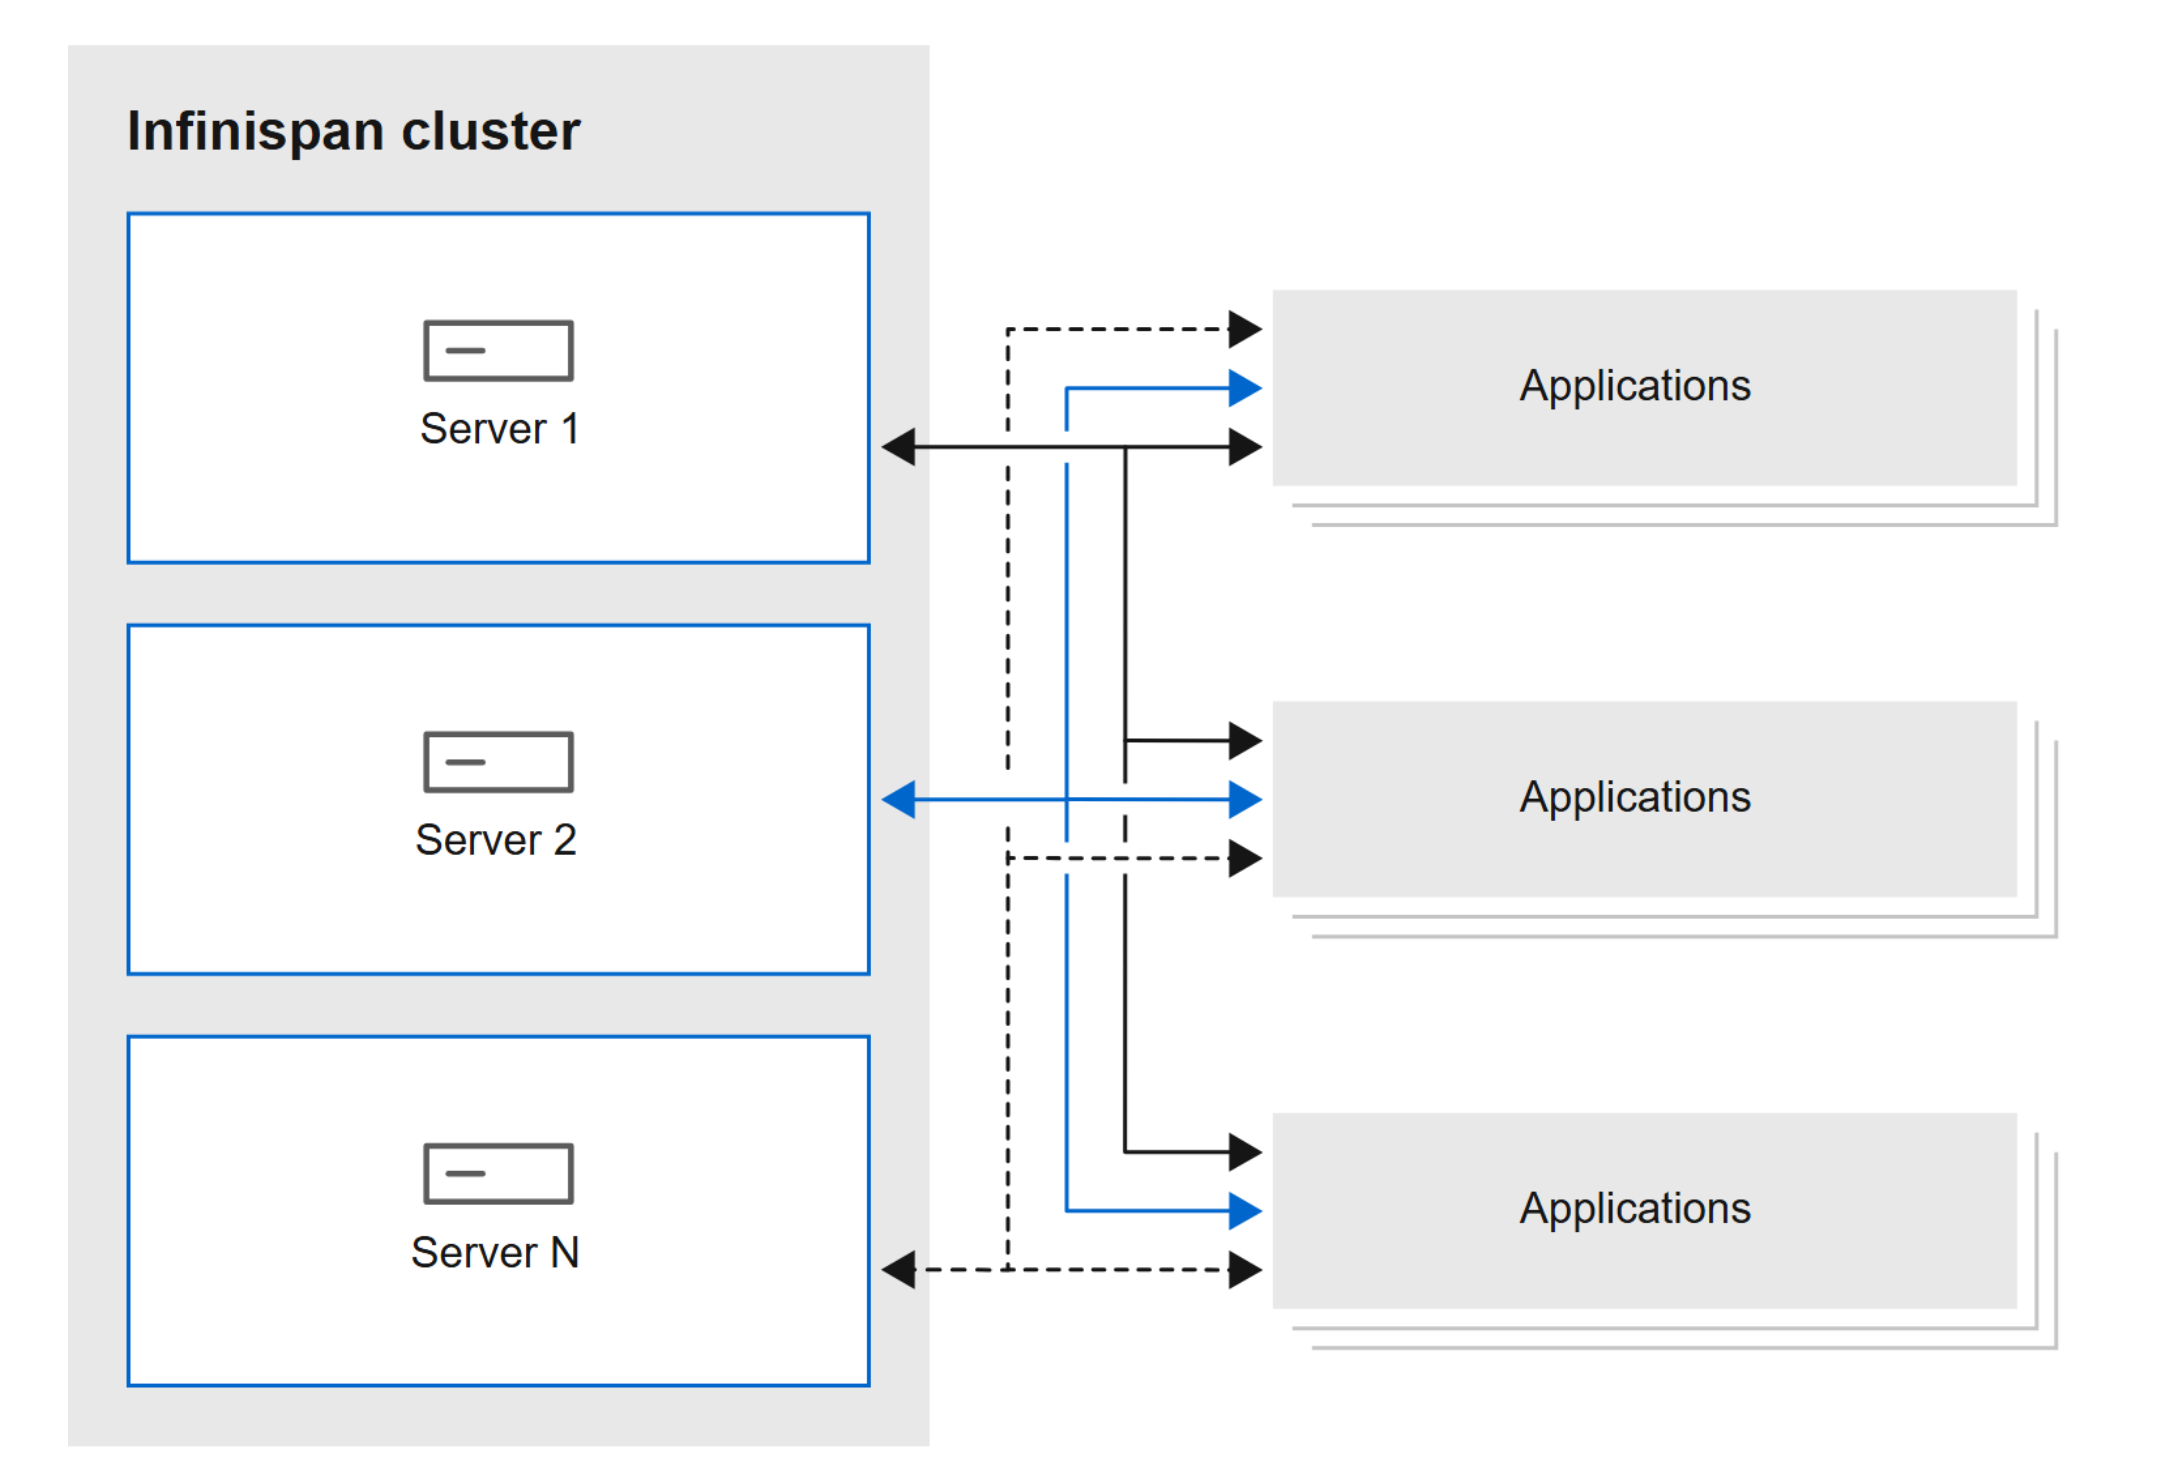
\includegraphics[width=0.85\textwidth]{figuras/infinispan-cluster.png}
\fonte{\citeonline{infinispan_tuning}}
\end{figure}

A distribuição de chaves entre nós segue o esquema de \emph{consistent hashing}, onde o conjunto de chaves é dividido em um número fixo de segmentos, definido por \texttt{numSegments}, e cada segmento é atribuído a uma lista de donos \revini{FUN-28}\cite[seção 2.2.2]{infinispan_configuring_15}\revfim{FUN-28}. \revini{FUN-29}O esquema padrão atribui as chaves aos mesmos nós em todos os \emph{caches}, desde que todos os \emph{caches} existam em todos os nós, ao custo de uma distribuição de carga levemente desigual \cite[seção 2.2.2]{infinispan_configuring_15}\revfim{FUN-29}; a variante ciente da topologia distribui as cópias por níveis topológicos como sites, racks e máquinas, para reduzir a chance de perda em falhas correlacionadas; e a variante de equilíbrio uniforme otimiza o balanceamento com a desvantagem de o resultado depender da ordem de entrada dos nós no \emph{cluster}. Quando a composição do \emph{cluster} muda, ocorre rebalanceamento, e segmentos são transferidos entre nós; durante a transição, mudanças de topologia podem causar repetições e mensagens adicionais para operações de leitura e escrita.

Nos modos \texttt{REPL\_SYNC} e \texttt{REPL\_ASYNC}, em contraste com a atribuição por segmentos própria dos modos distribuídos, cada nó mantém uma cópia completa de todas as entradas. A Figura~\ref{fig-datagrid-repl} representa esse comportamento em um \emph{data grid} replicado. Uma escrita submetida por um cliente, denotada \texttt{put()}, é aplicada em um nó e propagada aos demais pela replicação, assinalada como \texttt{REPL}, e cada nó atualiza os próprios índices locais a partir da atualização recebida. Uma consulta submetida por outro cliente, denotada \texttt{query}, é atendida localmente pelo nó que a recebe, pois todos os nós observam o mesmo conjunto de entradas depois de concluída a propagação. A figura torna visível o custo central da replicação assíncrona, dado que no intervalo entre a escrita local e a entrega da atualização aos demais nós as réplicas permanecem temporariamente divergentes.

\begin{figure}[htb]
\centering
\caption{Replicação de uma escrita entre os nós de um \emph{data grid}, com atualização dos índices por nó e leitura por consulta.}
\label{fig-datagrid-repl}
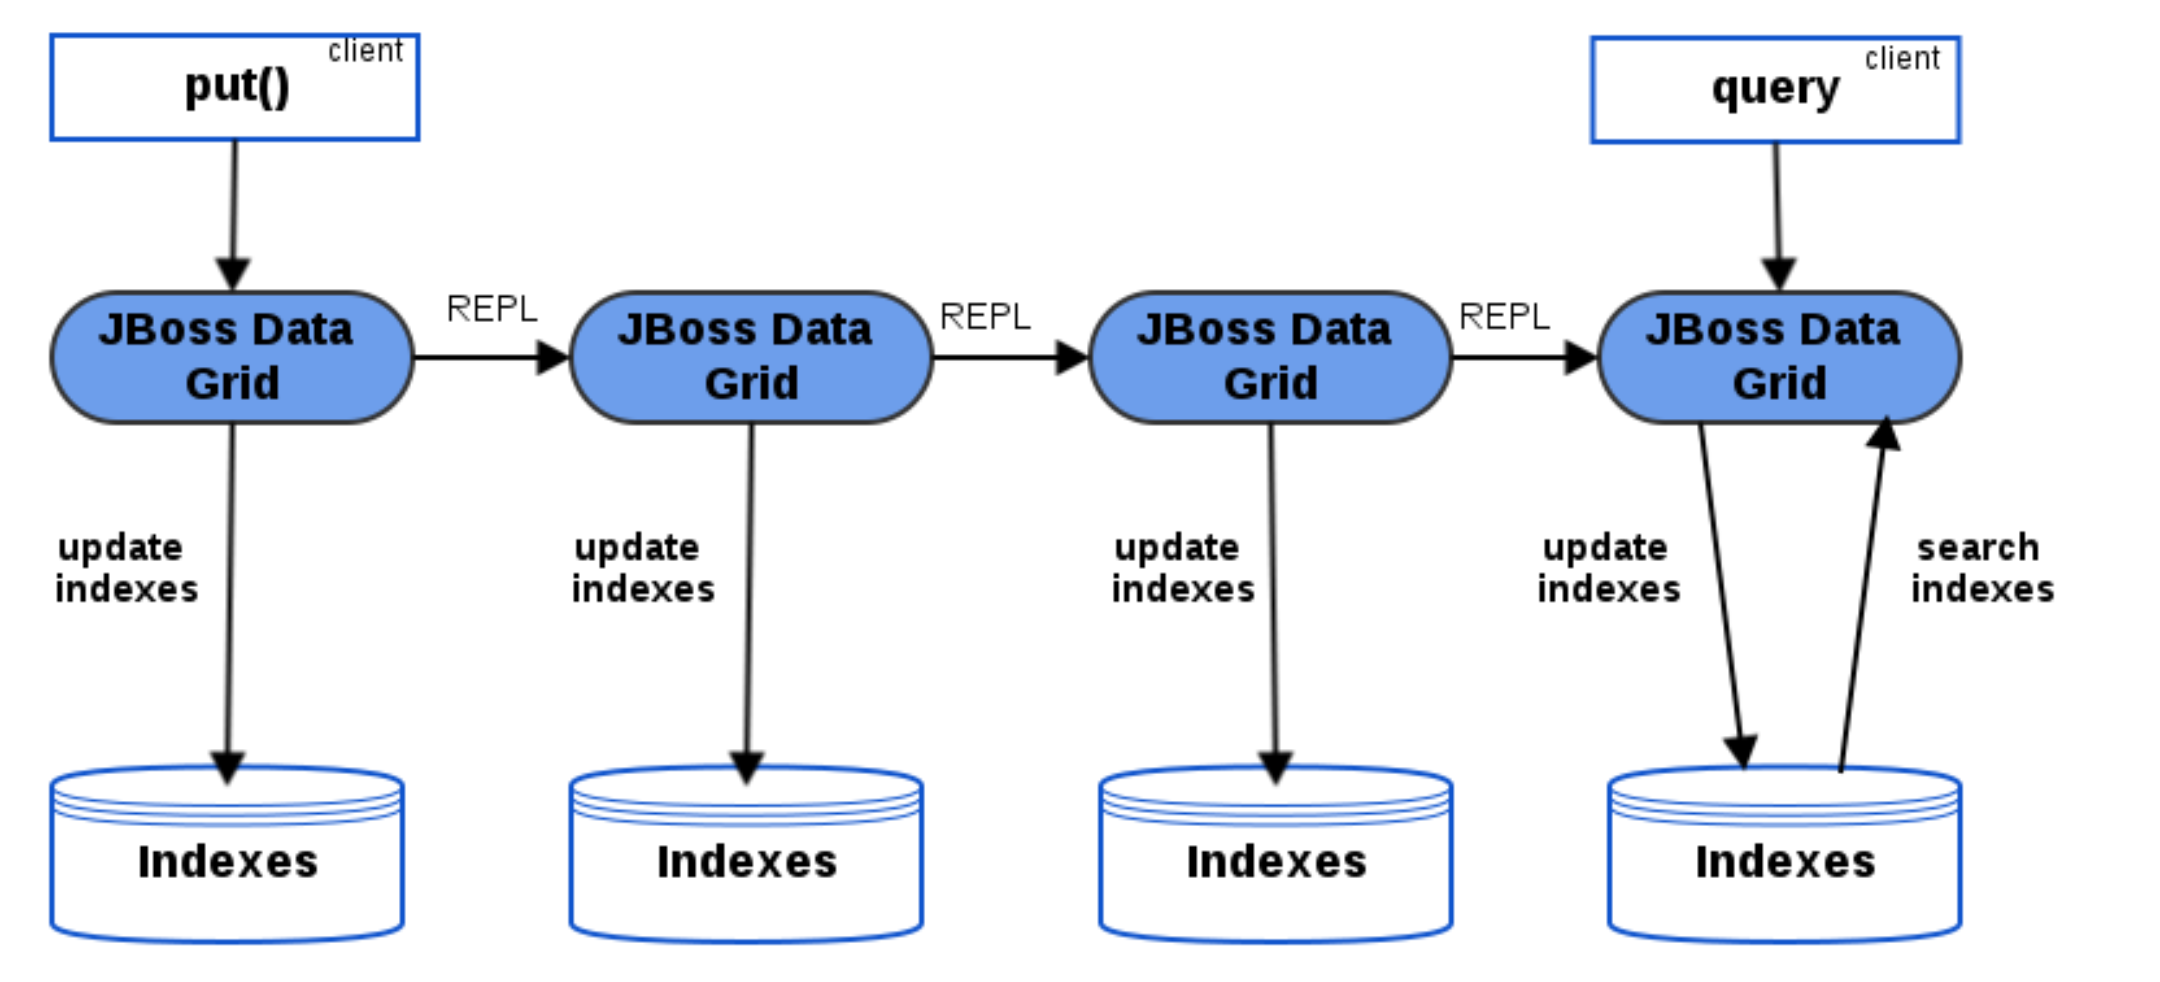
\includegraphics[width=0.95\textwidth]{figuras/datagrid-repl.png}
\fonte{\citeonline{redhat_datagrid_admin}}
\end{figure}

Para cenários multisite, a replicação \emph{cross-site}, ou seja, a replicação entre datacenters geograficamente distintos, permite cópias síncronas ou assíncronas entre \emph{clusters} separados \citep{infinispan_xsite}. A documentação registra duas regras importantes. A primeira é operacional: cópias assíncronas não adicionam latência às requisições do cliente, enquanto as síncronas introduzem o RTT entre sites em cada escrita, o que torna a opção assíncrona recomendada para configurações ativo-ativo em que dois sítios recebem escritas concorrentes. A segunda diz respeito à reconciliação: a detecção de conflitos por relógios vetoriais aciona políticas de resolução, com a política padrão usando comparação lexicográfica do nome do \emph{cluster}, e alternativas \texttt{ALWAYS\_REMOVE}, \texttt{PREFER\_NON\_NULL}, \texttt{PREFER\_NULL} ou implementação customizada pelo SPI \texttt{XSiteEntryMergePolicy}. A coleta de métricas operacionais segue documentação dedicada \citep{infinispan_metrics}: contadores por cache, indicadores de \emph{cluster}, sinais de \emph{cross-site}, latências médias e máximas, integração com JMX e exposição como Prometheus \citep{prometheus_docs}. Esses observáveis sustentam a instrumentação prevista para o controlador heurístico em etapa posterior.  Um ponto operacional ressaltado pela documentação merece registro: mesmo com replicação síncrona, caches distribuídos não são linearizáveis, dado que a escrita não é atômica entre os donos\revini{FUN-11} \cite[seção 2.2.1]{infinispan_configuring_15}\revfim{FUN-11}. Essa observação tem implicação direta sobre a formulação dos invariantes de sessão deste trabalho, dado que linearizabilidade não pode ser tomada como premissa nem no modo síncrono.

\section{Especificação formal e \emph{model checking}}
\label{sec-fund-formal}

A verificação por \emph{model checking} explora exaustivamente o espaço de estados de um modelo finito do sistema, com o objetivo de certificar a validade de propriedades declaradas ou produzir contraexemplos quando essas propriedades são violadas. \citet{yu_lamport_tla_modelchecking_1999} descrevem TLA+ como uma linguagem de especificação que combina a lógica temporal de ações TLA com lógica de primeira ordem completa e teoria dos conjuntos no estilo de Zermelo-Fraenkel. Uma especificação em TLA+ assume a forma canônica $\textit{Spec} \triangleq \textit{Init} \land \square [\textit{Next}]_v$, em que $\textit{Init}$ é um predicado sobre as variáveis $v$ que caracteriza os estados iniciais, $\textit{Next}$ é a relação de transição expressa como disjunção de ações, e $\square$ é o operador temporal que afirma que a fórmula a ele subordinada vale em todo estado da execução. Cada ação é um predicado sobre os valores das variáveis no estado corrente e no estado seguinte, denotadas $x$ e $x'$. Propriedades de invariância são fórmulas $\square \, P(v)$ que afirmam que todos os estados alcançáveis satisfazem $P$; propriedades temporais como $\square (P \Rightarrow \diamond Q)$ expressam restrições sobre sequências de estados e afirmam que todo $P$ é eventualmente seguido por um $Q$. O verificador TLC aceita um subconjunto de TLA+ adequado a descrições de sistemas reais, gera o grafo de estados acessíveis a partir dos estados iniciais \revini{FUN-30}por busca em largura\revfim{FUN-30}, mantém um conjunto de estados visitados por impressão digital de estado, e, quando encontra um estado que viola um invariante, retorna a sequência de transições que reproduz a violação. \citet{yu_lamport_tla_modelchecking_1999} \revini{FUN-31}registram o uso do TLC na especificação do protocolo de coerência de \emph{cache} de um novo multiprocessador da Compaq, com cerca de 1.800 linhas, na qual o verificador encontrou perto de duas dezenas de erros, dois deles presentes também na implementação em RTL, que foi corrigida \citep[seção 7]{yu_lamport_tla_modelchecking_1999}.\revfim{FUN-31}

A Figura~\ref{fig-tlc-estados} ilustra, em um exemplo mínimo com duas variáveis inteiras $x$ e $y$, a forma como o TLC percorre o espaço de estados. O estado inicial, definido por \textit{Init}, atribui o valor zero às duas variáveis. Cada aplicação da relação de transição \textit{Next} produz os estados sucessores admissíveis, e o não determinismo da relação faz um mesmo estado originar mais de um sucessor, como no ramo em que o estado com $x = 3$ dá origem a dois estados distintos após a segunda transição. O verificador repete esse passo sobre cada estado gerado e mantém o conjunto dos estados já visitados para não reexplorá-los. A verificação de um invariante avalia o predicado declarado em cada estado alcançado, e a primeira avaliação falsa interrompe a busca e devolve a sequência de transições que reproduz a violação.

\begin{figure}[htb]
\centering
\caption{Exploração do espaço de estados pelo verificador TLC, em que a relação de transição gera os estados sucessores a partir do estado inicial.}
\label{fig-tlc-estados}
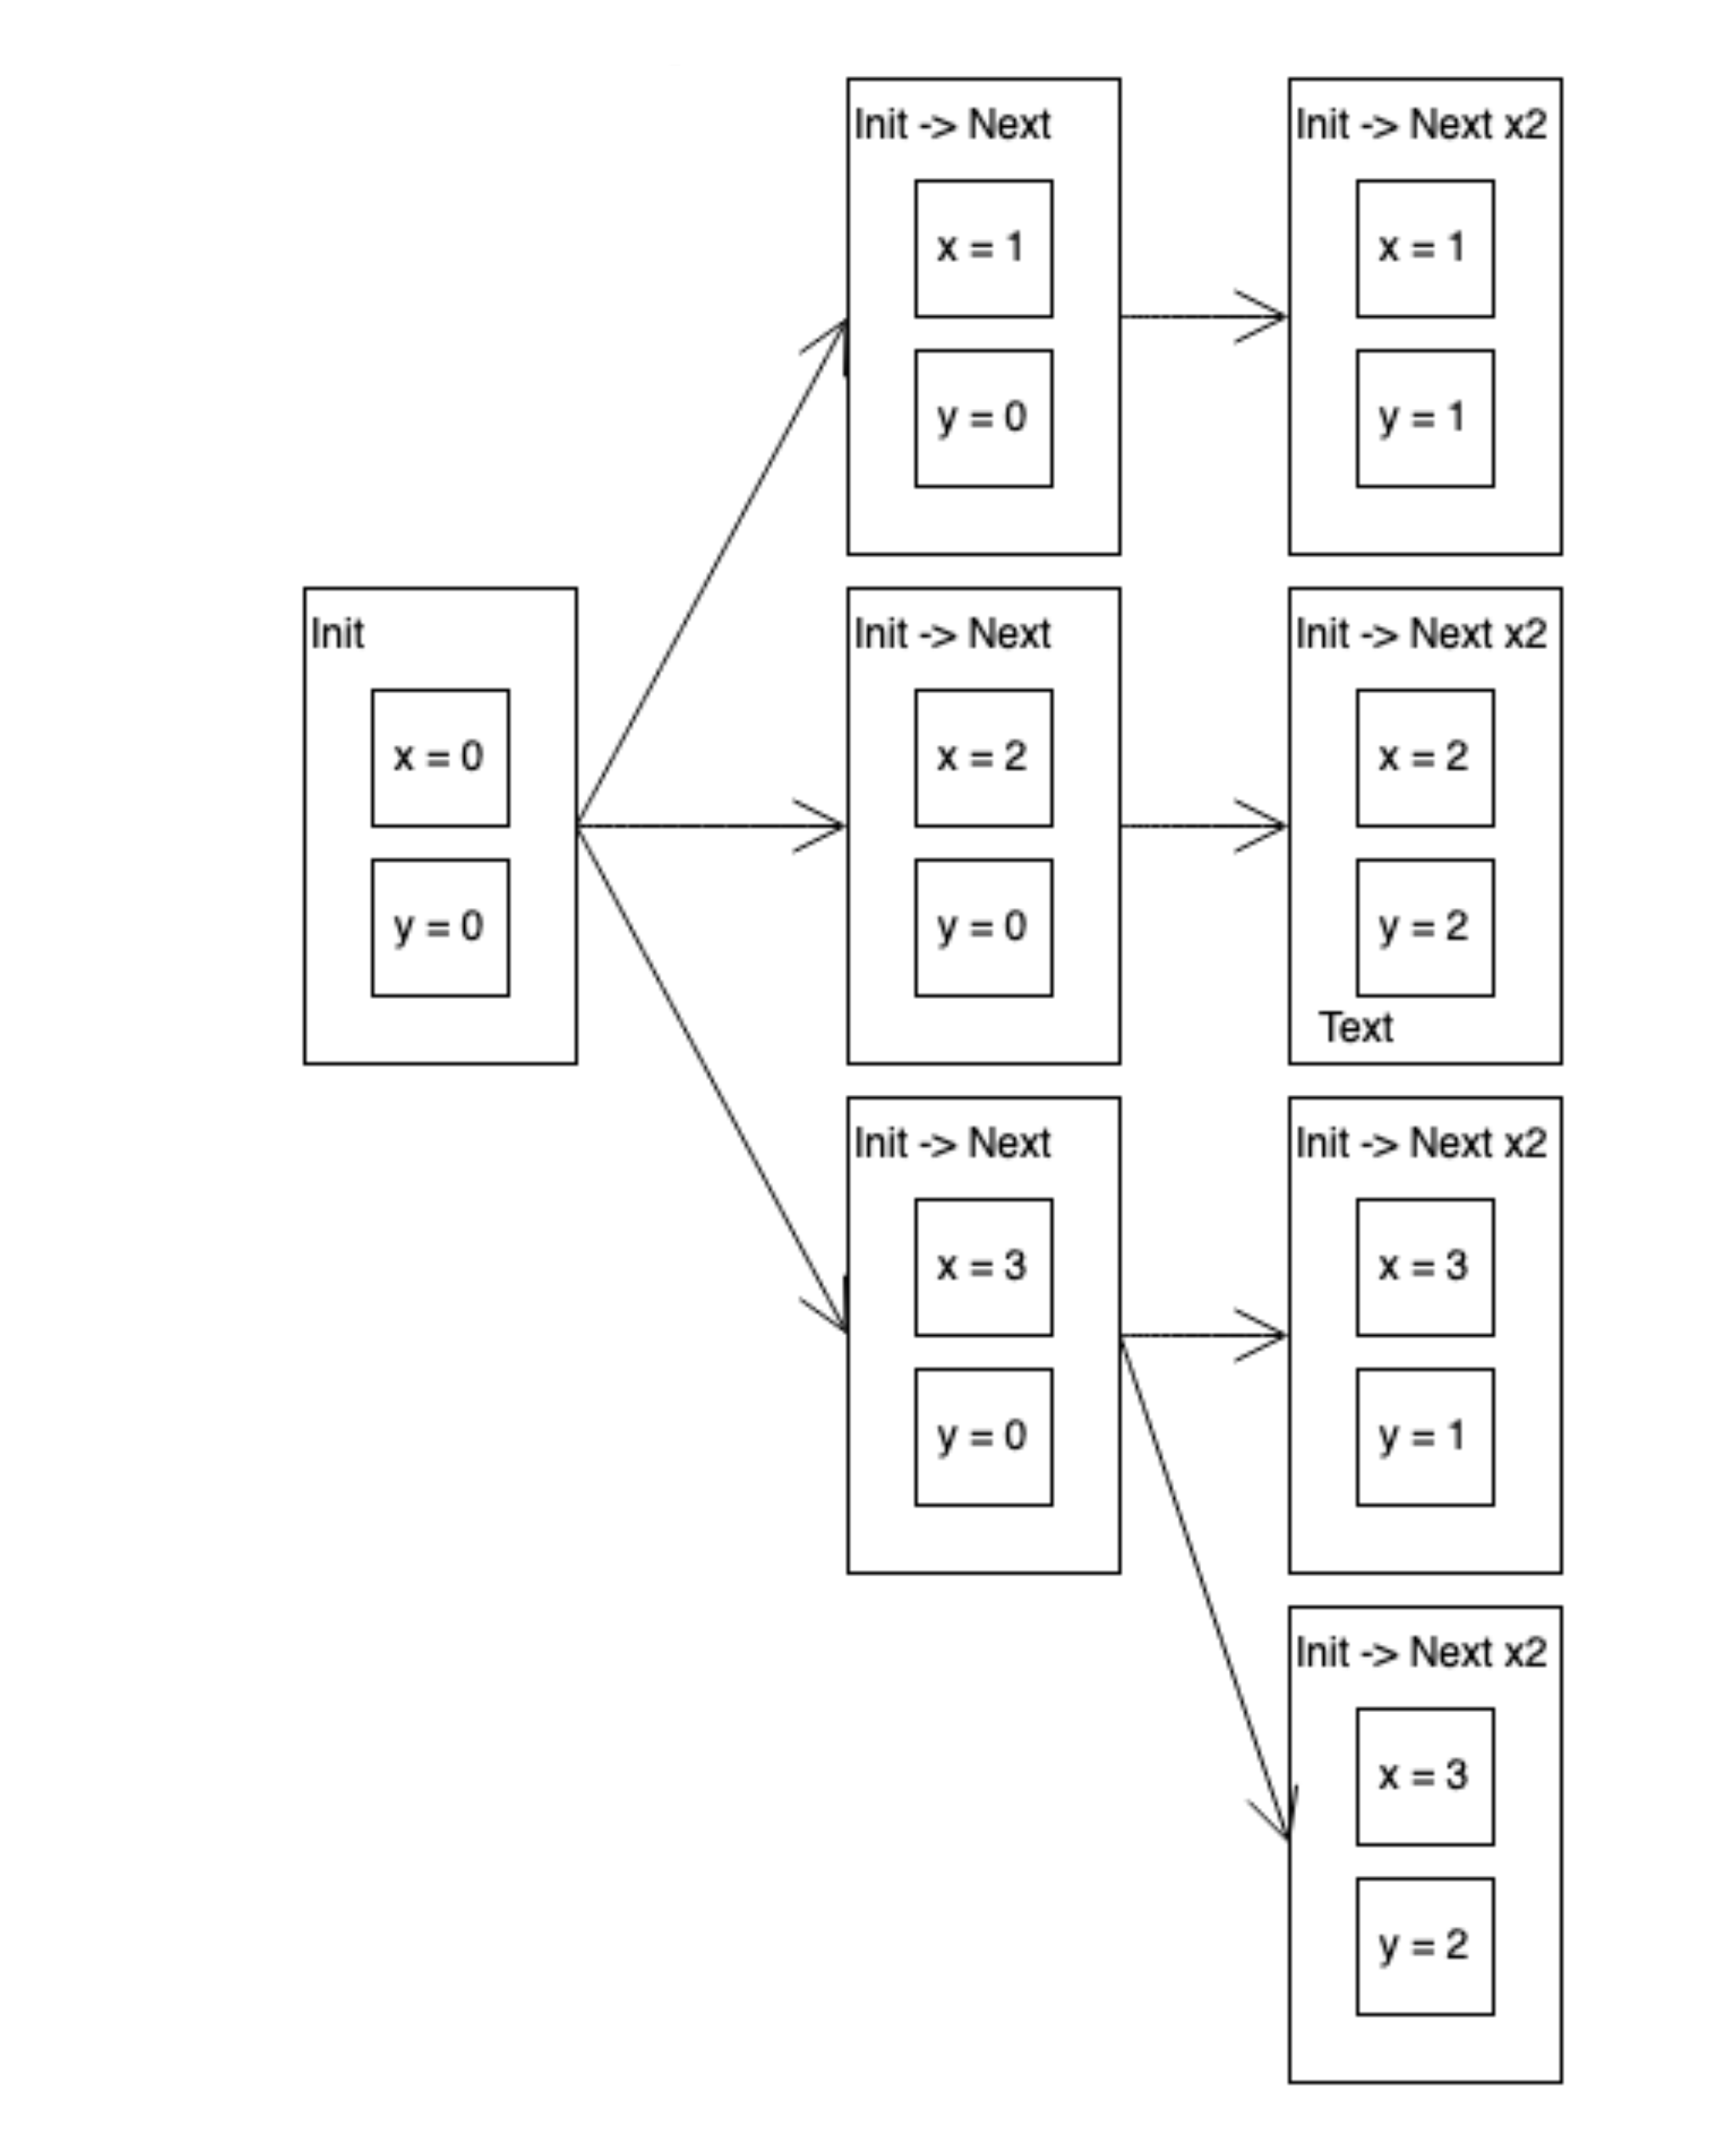
\includegraphics[width=0.62\textwidth]{figuras/tlc-estados.png}
\fonte{\citeonline{lee_tla_tlc_2021}}
\end{figure}

A representação eficiente do espaço de estados é o gargalo central da abordagem. \citet{yu_lamport_tla_modelchecking_1999} relatam estratégias para armazenar conjuntos de estados em disco e usar \revini{FUN-32}impressões digitais de 64 bits, únicas com alta probabilidade\revfim{FUN-32}, e essas opções determinam o tamanho dos modelos tratáveis. Em sistemas distribuídos, o espaço cresce com o número de nós, o tamanho da fila de mensagens em trânsito e a quantidade de tipos de evento, com explosão combinatória que motiva abstrações por simetria, por particionamento ou por redução parcial de ordem\revini{FUN-33} \citep{enea_must_2024}\revfim{FUN-33}. Daí a opção recorrente, no desenho de modelos formais para esses sistemas, por abstrações que mantenham a essência da concorrência sem replicar todos os detalhes da implementação. A aplicação industrial subsequente, com destaque para o registro de adoção pela Amazon Web Services, documenta a identificação de defeitos sutis em protocolos de replicação. \revini{FUN-12}\citet{newcombe_aws_formal_methods_2015}\revfim{FUN-12} relatam que a verificação formal encontrou, no projeto do DynamoDB, um defeito que poderia levar à perda de dados por meio de uma sequência de 35 passos envolvendo interações entre transações concorrentes, particionamento e recuperação, defeito que escapou a revisões extensivas de desenho, de código e a testes convencionais, e que motivou alteração no protocolo antes da implantação em produção.

A produção contemporânea estende a técnica em três direções. A primeira combina verificação formal e teste de implementações: um modelo formal guia testes incrementais sobre o sistema real, com o objetivo de aproximar o que foi verificado do que está executando, por instrumentação que mapeia transições do modelo a observações no código \citep{gao_mc_incremental_2025}. A segunda verifica diretamente protocolos distribuídos com semântica de mensagens assíncronas e falhas, em ferramentas projetadas para esse propósito; \revini{FUN-34}Must oferece uma interface de concorrência com vários modelos de comunicação, verifica os programas por redução parcial de ordem dinâmica e foi aplicada a sistemas de produção, como \emph{logs} replicados e protocolos de transação distribuída \citep{enea_must_2024}.\revfim{FUN-34} A terceira é a verificação probabilística de modelos: o resultado da análise é uma probabilidade de violação sob distribuições associadas a parâmetros do sistema, \revini{FUN-35}e aplica-se a decisões de escalonamento horizontal em bancos NoSQL ciente de custo \citep{naskos_probabilistic_mc_2017}\revfim{FUN-35}. A escolha da ferramenta para este trabalho, entre TLA+/TLC e as alternativas, fica detalhada e justificada na Seção~\ref{sec-escolha-ferramenta}.

\revini{FUN-13}A verificação exaustiva só é tratável com cardinalidades pequenas, e a pertinência desse recorte tem apoio empírico. \citet{yuan_simple_testing_2014}, ao analisar falhas reportadas em sistemas distribuídos de produção, constatam que \revini{FUN-36}98\% delas\revfim{FUN-36} se manifestam com três nós ou menos. A observação sustenta tanto os modelos com duas ou três réplicas verificados pelo TLC quanto o \emph{cluster} experimental de três nós, embora não garanta que todo defeito do protocolo apareça nessas cardinalidades.\revfim{FUN-13}

\section{Latência de cauda, objetivos de nível de serviço e observabilidade}
\label{sec-fund-slo}

A distribuição de latência de um serviço composto por muitos componentes tem cauda longa, e o impacto dessa cauda sobre o tempo total observado pelo usuário é desproporcional ao seu peso na distribuição. \citet{dean_barroso_tail_2013} ilustram o fenômeno com um caso em que a latência típica de uma requisição fica em torno de $10$ milissegundos, com 1\% das requisições demorando mais de $1$ segundo (cem vezes a típica). Em sistemas de \emph{fan-out}, em que uma requisição do usuário se decompõe em $n$ requisições independentes a componentes distintos e depende da resposta mais lenta, a probabilidade de pelo menos uma resposta cair na cauda cresce rapidamente com $n$: se a probabilidade de uma resposta individual ser lenta é $p = 0{,}01$, a probabilidade de pelo menos uma resposta lenta em $n = 100$ componentes é $1 - (1-p)^n \approx 0{,}63$, ou seja, 63\% das requisições do usuário tocam pelo menos uma resposta na cauda. \revini{FUN-37}As fontes de variabilidade apontadas pelos autores incluem disputa por recursos compartilhados na máquina e na rede, atividades de manutenção em segundo plano, como a coleta de lixo, filas em servidores e comutadores e mecanismos de economia de energia do \emph{hardware}.\revfim{FUN-37} Por isso, os percentis p95 e p99, e em sistemas críticos o p99,9, são as métricas primárias em vez da média. As técnicas de tolerância à cauda incluem requisições redundantes (\emph{hedged requests}), em que o cliente envia uma cópia secundária após $T$ milissegundos de espera, com $T$ tipicamente fixado no p95 esperado, e cancela a réplica que perde a corrida; e requisições atadas (\emph{tied requests}), em que servidores que recebem cópias se comunicam para cancelar a duplicata assim que um deles começa o atendimento. \revini{FUN-38}Esperar até o p95 limita a carga adicional das requisições redundantes a cerca de 5\%, e em um exemplo dos autores 2\% de requisições a mais reduziram o p99,9 de 1.800 para 74 milissegundos; nas requisições atadas, a sobrecarga medida em uso de disco ficou abaixo de 1\%.\revfim{FUN-38}

A formulação dessas metas como objetivos de nível de serviço segue prática consolidada \citep{google_sre_slo}. Um indicador de nível de serviço (SLI) é definido como uma medida quantitativa de algum aspecto do nível de serviço fornecido. Um objetivo de nível de serviço (SLO) é um valor-alvo, ou intervalo de valores, para o nível de serviço medido por um SLI, expresso como $\text{SLI} \le \text{alvo}$ ou $\text{limite inferior} \le \text{SLI} \le \text{limite superior}$; um exemplo prescrito pela literatura é ``99\% das chamadas de \texttt{Get} completam em menos de 100 milissegundos''. Um acordo de nível de serviço (SLA) é um contrato explícito ou implícito com os usuários, com consequências do cumprimento ou descumprimento dos SLO nele contidos. \revini{FUN-39}O orçamento de erros é a taxa com que os SLOs podem deixar de ser cumpridos, acompanhada diariamente ou semanalmente, e seu consumo funciona como entrada para decisões operacionais.\revfim{FUN-39} Sobre agregação, médias simples obscurecem detalhes importantes, e a combinação de mediana, p99 e p99,9 caracteriza a forma da distribuição com mais fidelidade do que qualquer estatística única.

A pesquisa específica em armazenamentos chave-valor estuda como reduzir a cauda de latência por agendamento de consultas, com algoritmos que tratam heterogeneidade de operações \citep{jaiman_tailx_2020, benmokhtar_taming_tail_2021}, e estende esse trabalho em versão expandida com avaliação ampla de cenários \citep{benmokhtar_scheduling_2024}. A observabilidade operacional encontra-se sistematizada em estudos sobre rastreamento e análise em microsserviços, que documentam práticas de instrumentação, retenção e análise de sinais sobre execuções distribuídas \citep{li_observability_2021}. No Infinispan, os contadores e indicadores publicados conforme a documentação de métricas dão acesso aos observáveis necessários para correlacionar variações de latência e eventos operacionais com violações de invariantes \citep{infinispan_metrics}.

\revini{FUN-14}\label{sec-fund-avaliacao}A avaliação experimental de sistemas computacionais precisa lidar com a variabilidade entre execuções. \citet{georges_jvm_statistics_2007} mostram que o desempenho de programas Java não é determinístico, por efeito de fatores como a compilação dinâmica, a coleta de lixo e o escalonamento de \emph{threads}, e que metodologias de avaliação sem rigor estatístico podem levar a conclusões enganosas. Para médias estimadas a partir de poucas execuções, o intervalo de confiança usa a distribuição $t$ de \citet{student_probable_error_1908}. \citet{hoefler_belli_benchmarking_2015} sistematizam regras para relatar resultados de desempenho, entre elas tratar a execução repetida como unidade de medida, reportar a variabilidade por intervalos de confiança e preferir procedimentos não paramétricos quando os dados não seguem distribuição normal. Para estatísticas sem distribuição amostral conhecida, como os percentis de latência, o \emph{bootstrap} aproxima essa distribuição por reamostragem dos dados observados, e o intervalo percentil toma os quantis da distribuição reamostrada \citep{efron_tibshirani_bootstrap_1993}. O teste de \citet{mann_whitney_1947} compara duas amostras sem supor normalidade e verifica se uma das variáveis tende a assumir valores maiores que a outra. Para proporções, \citet{brown_cai_dasgupta_binomial_2001} mostram que o intervalo padrão baseado na aproximação normal da binomial tem cobertura errática, que se afasta do nível nominal de modo irregular, o que recomenda cautela no uso dessa aproximação.\revfim{FUN-14}

\revini{FUN-15}Quando o mesmo pesquisador desenha, executa e analisa um experimento, decisões tomadas depois de ver os dados podem ser apresentadas, sem intenção, como previsões. \citet{nosek_preregistration_2018} defendem o pré-registro como resposta: hipóteses, desfechos e plano de análise são fixados antes da coleta, o que separa a análise confirmatória da exploratória.\revfim{FUN-15}

\revini{FUN-16}A estimativa de energia parte de modelos de potência por utilização. \citet{fan_power_provisioning_2007} observam que a potência de um servidor varia de forma aproximadamente linear com a utilização da CPU, o que permite estimá-la por $P(u) = P_\text{ocioso} + (P_\text{máx} - P_\text{ocioso}) \cdot u$, em que $u$ é a utilização. \citet{barroso_holzle_energy_proportional_2007} mostram que servidores consomem parcela elevada da potência de pico mesmo quando ociosos e passam a maior parte do tempo em utilização baixa ou moderada, de modo que a parcela ociosa pesa na energia por operação. Em máquinas virtuais, a potência não pode ser medida diretamente no \emph{hardware} e precisa ser estimada por modelos alimentados por contadores de uso de recursos \citep{kansal_vm_power_2010}. No Linux, a interface de grupos de controle versão 2 (cgroup v2) expõe o tempo de CPU acumulado por grupo de processos, o que permite atribuir o tempo de CPU a cada \emph{container} \citep{linux_cgroup_v2}.\revfim{FUN-16}

\section{Sistemas autoadaptativos e controle por realimentação}
\label{sec-fund-adapt}

Um sistema autoadaptativo monitora seu próprio comportamento, analisa desvios em relação a metas e atua sobre parâmetros configuráveis para retornar à região operacional. Em ambientes de nuvem, a literatura organiza essas atividades por meio de taxonomias e revisões que descrevem mecanismos de elasticidade sob a ótica da teoria de controle, com critérios como estabilidade, tempo de acomodação e prevenção de oscilação \citep{ullah_control_elasticity_2018}. Trabalhos de implementação demonstram autoescala em armazenamentos de nuvem hierárquicos \citep{wu_anna_autoscale_2020} e gestores proativos de elasticidade autotreinados \citep{liu_onlineelastman_2017}. Para o desenho de controladores adaptativos, a literatura discute mecanismos de garantia que combinam evidência empírica e propriedades formais \citep{gambi_assurance_selfadaptive_2013}, e propõe políticas de auto-gestão baseadas em objetivos de alto nível em sistemas distribuídos \citep{rosa_selfmgmt_2013}. \revini{FUN-17}A referência conceitual comum a esses trabalhos é o laço monitorar-analisar-planejar-executar sobre uma base de conhecimento (MAPE-K), do gerente autônomo descrito por \citeonline{kephart_chess_autonomic_2003}.\revfim{FUN-17}

O controlador previsto para etapa posterior deste trabalho é heurístico, com regras determinísticas e mecanismos de histerese para evitar oscilação, e atua sobre um conjunto finito de configurações pré-definidas.  A escolha do desenho heurístico, em lugar de soluções baseadas em aprendizado de máquina ou em controle ótimo, segue dois critérios. O primeiro é a auditabilidade das decisões: cada ação aplicada pelo controlador pode ser rastreada para a regra que a motivou, o que sustenta análise de causa raiz após qualquer ocorrência. O segundo é a tratabilidade formal: regras determinísticas com observáveis bem-definidos prestam-se à análise pelo modelo formal do trabalho, conforme delineado no Capítulo~\ref{cap-metodologia}. \revini{FUN-40}\citet{ullah_control_elasticity_2018} apontam que controladores de elasticidade precisam evitar oscilação e se acomodar rapidamente após perturbações, e três fenômenos operacionais merecem atenção.\revfim{FUN-40} O primeiro é a alternância rápida entre estados de configuração, que introduz instabilidade e impede que qualquer estado se mantenha por tempo suficiente para produzir efeito. O segundo é a sobre-resposta, em que a reação supera a correção necessária e leva o sistema a oscilar em torno do valor-alvo. O terceiro é o atraso de fase, em que a ação chega depois da janela em que produziria efeito. Regras com histerese e limites de taxa de mudança são respostas diretas a esses três fenômenos.

\section{Gerência de sessão como domínio}
\label{sec-fund-sessao}

A gerência de sessão constitui o estudo de caso do trabalho. O ciclo de vida de uma sessão compreende criação, validação, renovação, invalidação e bloqueio, sobre uma identidade autenticada. \revini{FUN-19}A literatura normativa estabelece propriedades que esse ciclo deve satisfazer. A publicação SP 800-63B-4 do NIST, que substituiu a versão de 2017, define níveis de garantia do autenticador com prazos de reautenticação próprios de cada nível, trata da gerência de sessão em seção normativa, na qual exige que os segredos de sessão sejam invalidados no \emph{logout}, e exige a limitação do número de tentativas de autenticação malsucedidas, o chamado \emph{rate limiting} \cite[seções 2, 3.2.2 e 5]{nist_sp_800_63b4_2025}. Essas duas exigências fundamentam, respectivamente, a irreversibilidade da invalidação e o par formado pelo contador de tentativas e pelo bloqueio da identidade, objetos dos invariantes deste trabalho.\revfim{FUN-19}

A Figura~\ref{fig-sessao-ciclo} sintetiza o percurso de uma sessão autenticada quando o estado é externalizado para um repositório compartilhado. O usuário inicia o fluxo ao submeter credenciais em uma operação de \emph{login}, que o serviço de \emph{backend} autentica; confirmada a identidade, o serviço cria a sessão, registra-a no repositório de sessões e devolve ao cliente um \emph{cookie} que carrega apenas o identificador da sessão. Nas requisições seguintes, o cliente reapresenta esse \emph{cookie}, e o serviço valida a sessão por consulta ao repositório antes de produzir a resposta. A figura evidencia que a correção observada pelo usuário depende do estado mantido no repositório, e essa camada, quando replicada de forma assíncrona, expõe os invariantes de sessão às condições de falha tratadas neste trabalho.

\begin{figure}[htb]
\centering
\caption{Ciclo de vida de uma sessão autenticada com estado externalizado em repositório de sessões compartilhado.}
\label{fig-sessao-ciclo}
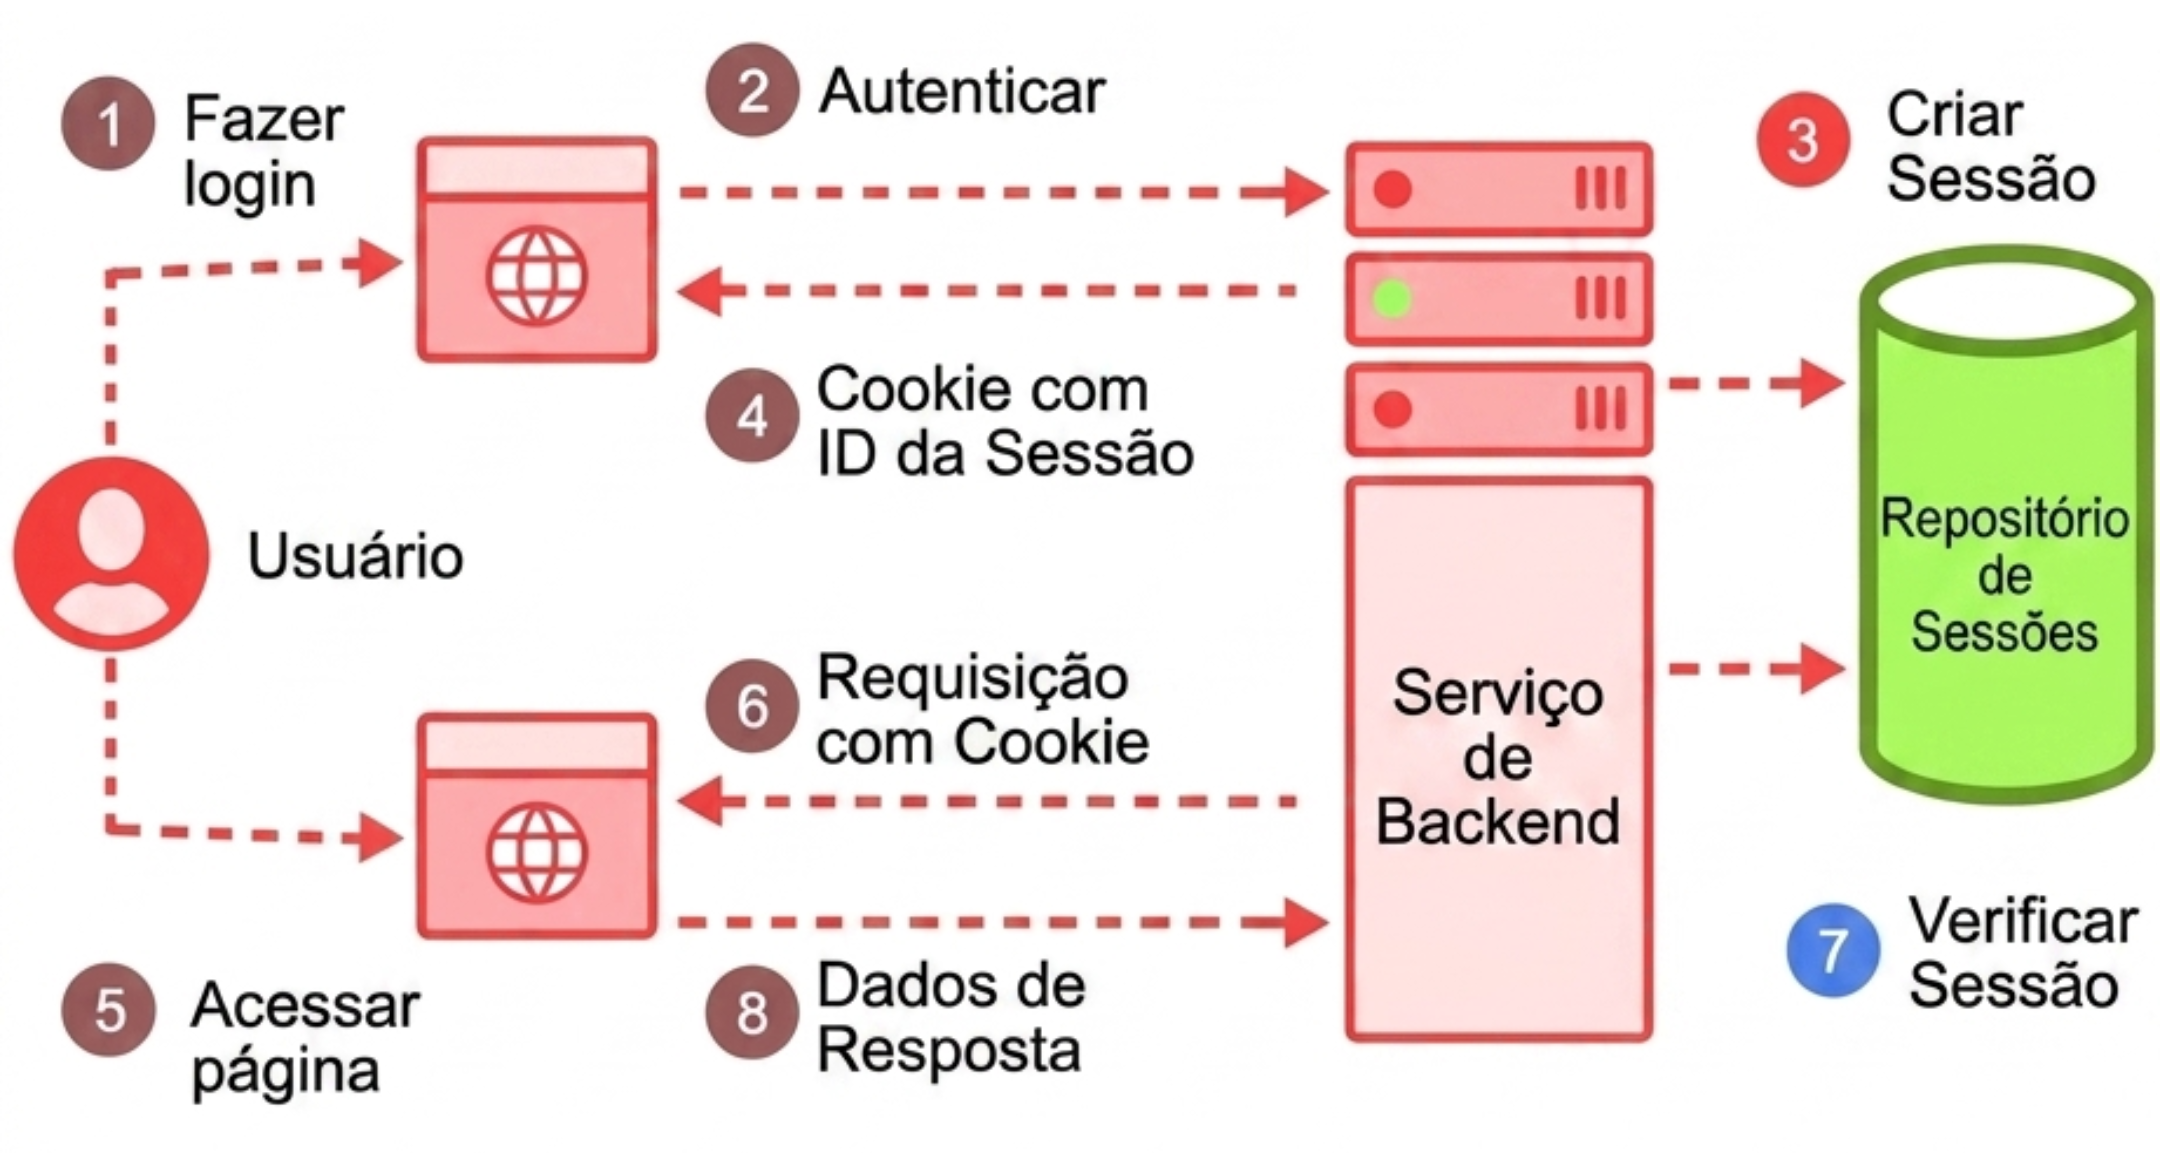
\includegraphics[width=0.9\textwidth]{figuras/sessao-ciclo.png}
\fonte{O autor}
\end{figure}

O \emph{OWASP Session Management Cheat Sheet} \citep{owasp_session_mgmt_cheatsheet} traduz essas exigências em requisitos operacionais sobre identificadores e atributos de sessão. O identificador de sessão deve ter pelo menos 64 bits de entropia, gerados por um gerador pseudoaleatório criptograficamente seguro, e deve evitar conteúdo significativo, ou seja, qualquer informação que permita a um observador deduzir o estado da sessão. Sobre o tempo de vida, três mecanismos complementares são prescritos: o tempo-limite absoluto define o tempo máximo de existência da sessão; o tempo-limite por inatividade encerra a sessão após inatividade; o tempo-limite de renovação rotaciona o identificador em intervalos regulares para reduzir a janela de exploração de identificadores capturados. A invalidação deve ser feita no servidor e no cliente, e o identificador deve ser regenerado após qualquer mudança de privilégio, em particular após a autenticação, para impedir ataques de fixação de sessão (\emph{session fixation}). Os atributos do \emph{cookie} devem incluir \texttt{Secure}, \texttt{HttpOnly}, \texttt{SameSite} e o prefixo \texttt{\_\_Host-}, para mitigar exposição em canal não seguro, acesso por código executado no cliente e envio em requisições de origem distinta.

\revini{FUN-41}Externalizar o estado de sessão em um IMDG ou armazenamento chave-valor aplica essa separação entre computação sem estado e armazenamento com estado \citep{armbrust_cloud_2010}: múltiplas instâncias servem requisições de um mesmo cliente sob balanceamento de carga.\revfim{FUN-41} A externalização desacopla o estado do nó que atende à requisição, com o ganho de continuidade em \emph{failover} e o custo da exposição aos efeitos da replicação assíncrona descritos na Seção~\ref{sec-fund-distrib}. A combinação dessas duas camadas, exigências normativas e operacionais, justifica a escolha de irreversibilidade de invalidação, consistência de bloqueio e monotonicidade de contadores como invariantes alvo deste trabalho.